\documentclass[12pt]{article}

\usepackage{float}
\usepackage{fancyhdr}
\usepackage{amsmath}
\usepackage{amsthm}
\usepackage{mathrsfs}
\usepackage{graphicx}
\usepackage{graphics}
\usepackage{subcaption}
\usepackage{hyperref}
\usepackage{wrapfig}
\usepackage{arydshln}
\usepackage{multirow} 
\usepackage{tikz}
\usepackage[natbib=true,
    style=numeric,
    sorting=none]{biblatex}
\addbibresource{bibi.bib}
\setkeys{Gin}{draft=false}

\begin{document}
\begin{titlepage}
	\centering
	{\textsc{University of Bonn} \par}
	\vspace{1cm}
	{\Large \textsc{Lab report}\par}
	\vspace{1.5cm}
	{\huge\bfseries Radio astronomical observing course\par}
	\vspace{2cm}
	{\Large\itshape Wajdee Chayeb \\
	MohammadReza Torkamani\par}
	\vfill
	Tutors:\par
	Jacob Cardinal Tremblay\\
	Alina Manthei

	\vfill

% Bottom of the page
	{\large \today\par}
\end{titlepage}

\section{Introduction}
The aim of this experiment is to understand the functionality of radio observation, study the electronics of a radio telescope, and subsequently observe and evaluate the resulting data. 
We observe a galaxy as well as signals of two different pulsars using the 25-m Stockert radio telescope. We first calibrate the telescope by observing a very bright source, then a galaxy is observed to determine its HI flux and estimate its mass. Finally, By calculation of the dispersion measure of a pulsar, the distance of it will be measured.

\section{Radio Telescopes}
Radio telescopes are specialized antennas and receivers used to detect and collect radio waves coming from astronomical objects \cite{fundamentals}. They are the main tools used in the field of radio astronomy and differ in type according to the aim of usage.  Since the range of frequencies in the electromagnetic spectrum, making up the radio spectrum, is very large, the types of antennas used vary in configuration, size, and design. In this report, we limit our discussion only to single-dish antennas, parabolic dish antennas, which dominate at shorter wavelengths of the radio regime. A parabolic antenna uses a parabolic reflector to direct the radio waves and has the advantage of high directivity and achieving high gain, producing the narrowest bandwidths \cite{antennabook}. An example is depicted in Figure \ref{fig2.1}. The size of a the dish determines the resolution of the telescope, which is given similar to that of optical telescopes as \cite{lecturenote}:
\begin{equation}
    HPBW = 1.22 \frac{\lambda}{D}
\end{equation}

Where HPBW is the half-power beam with, the ability to separate two unresolved sources, given in units of radians. $\lambda$ is the wavelength of incoming radiation and D is the diameter of the dish.

\begin{figure}[H]
\centering
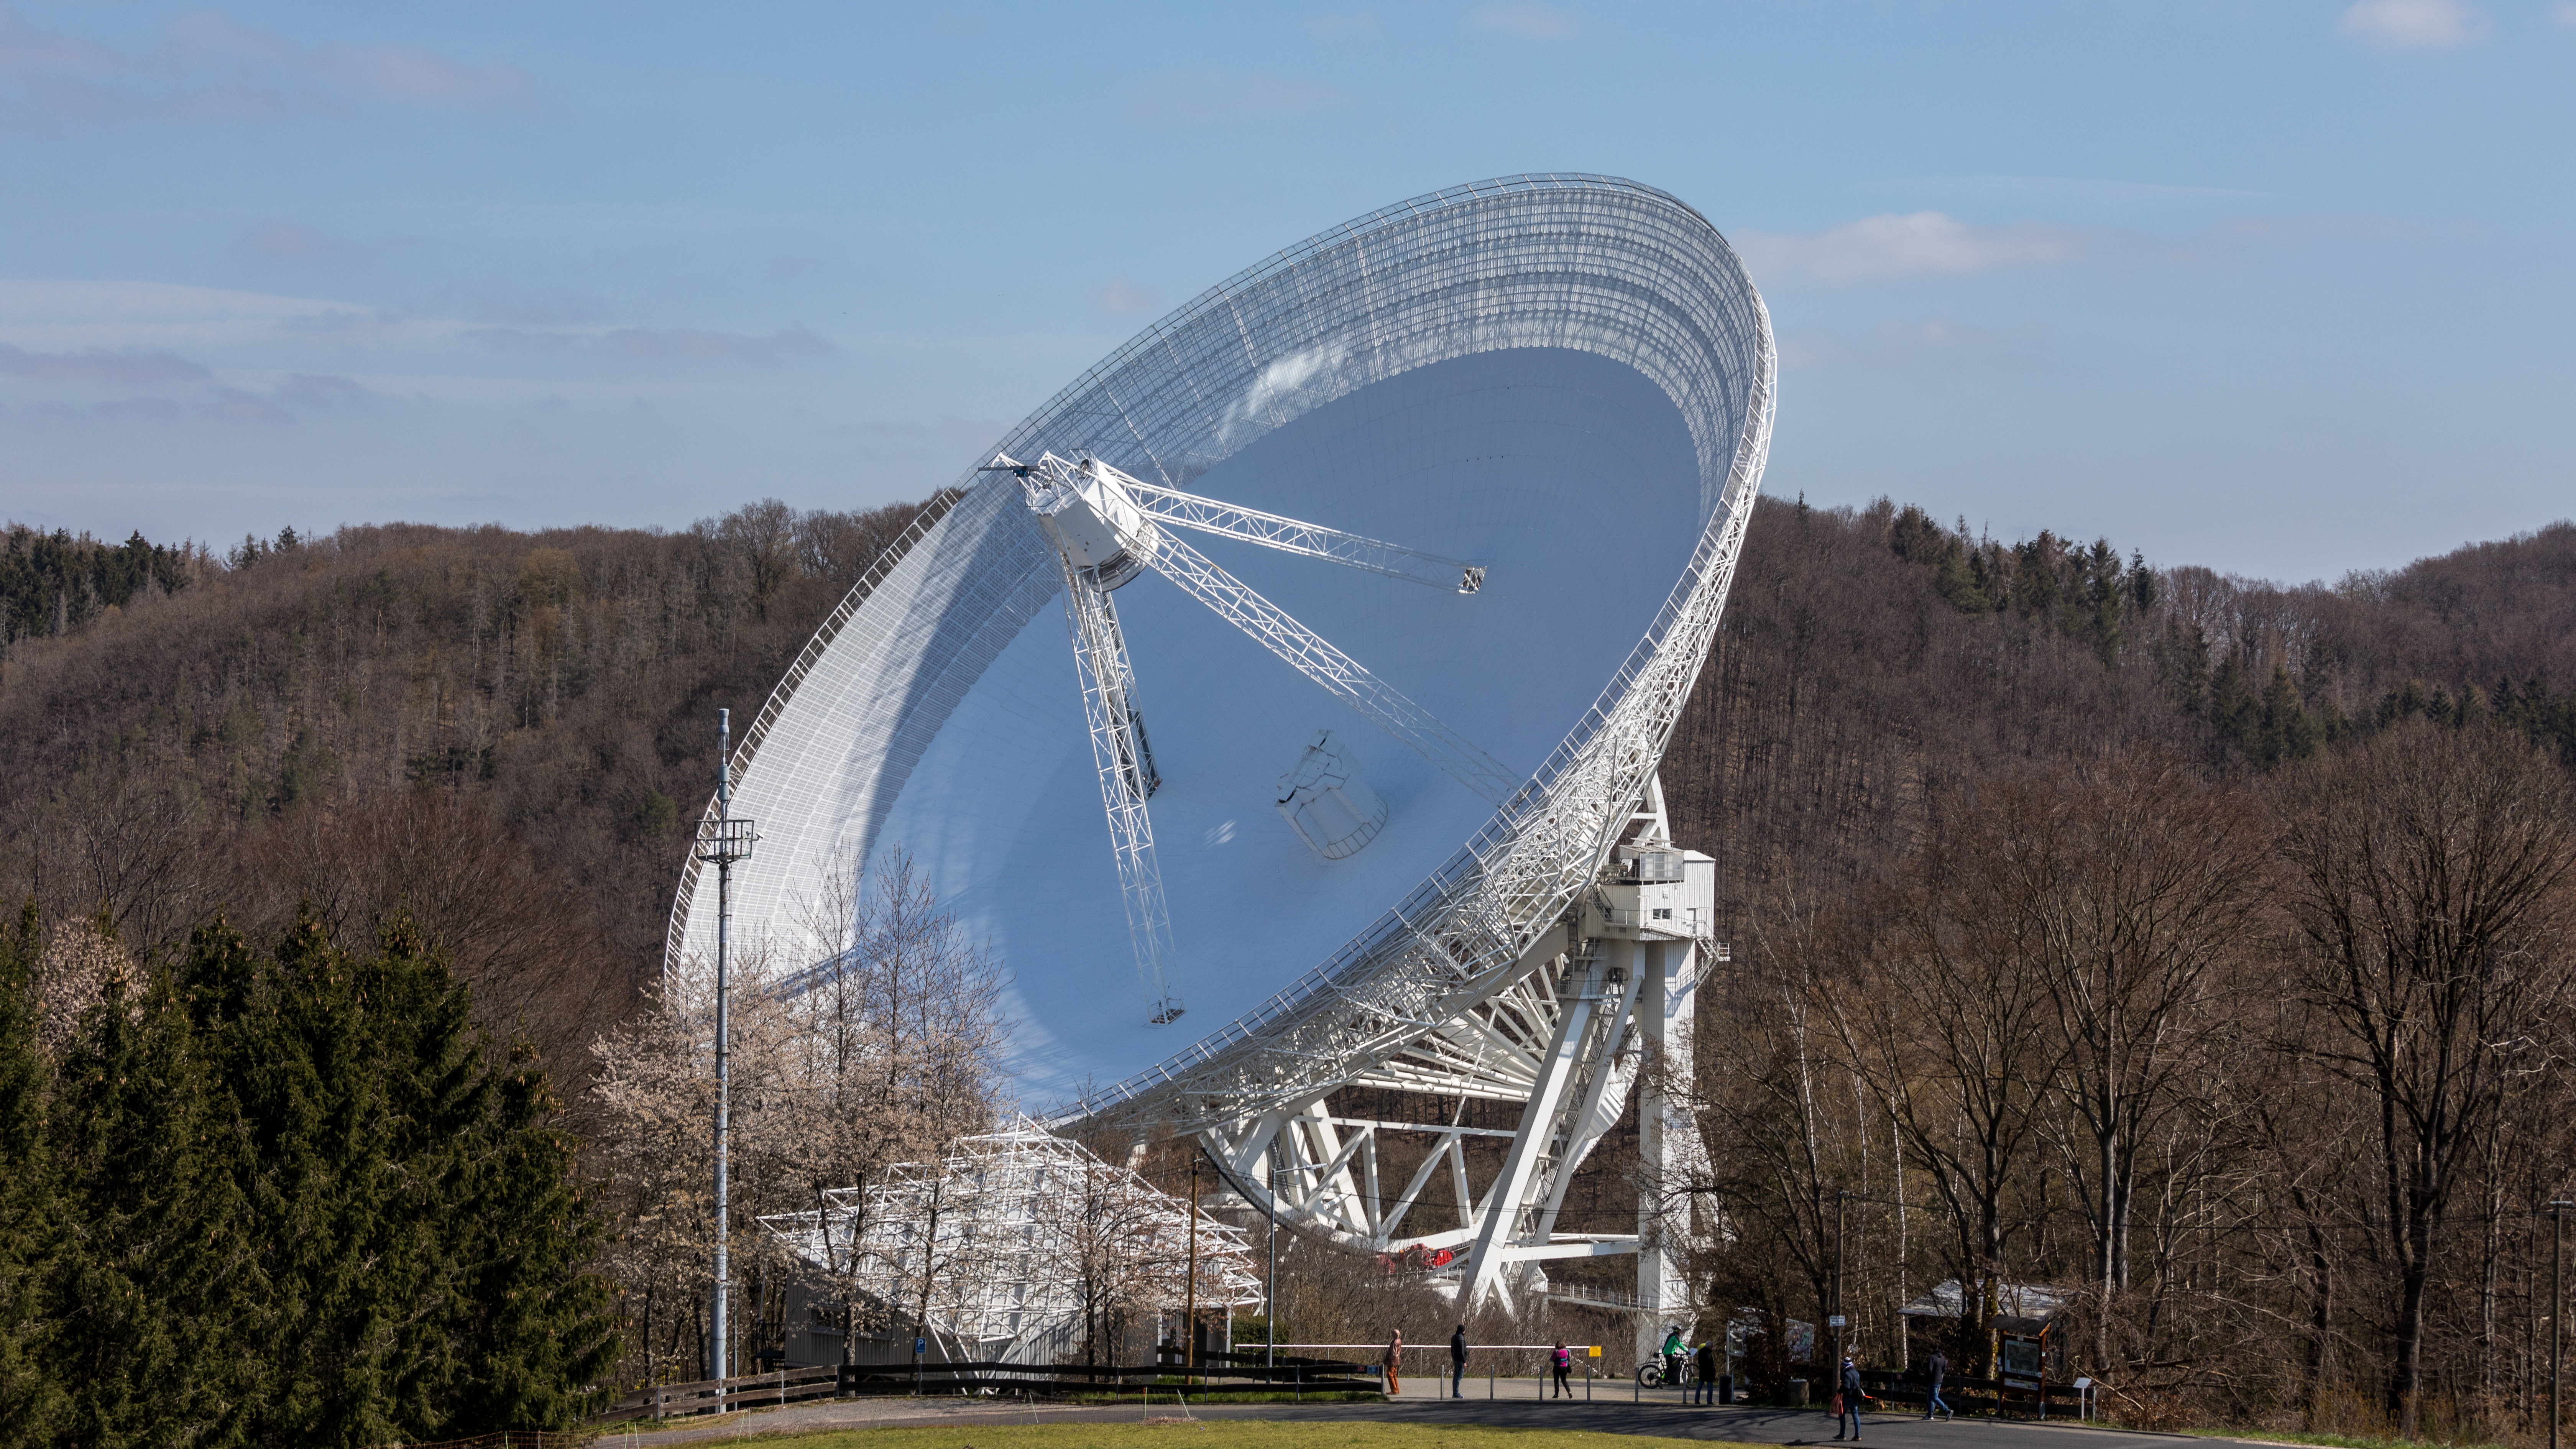
\includegraphics[scale=0.2]{fig/telescope.jpg}
\caption{A picture of the 100-m radio telescope Effelsberg, Germany. Image credit: \cite{effelsberg}}
\label{fig2.1}
\end{figure} 

    \subsection{Construction Principles \& Geometry}
    A single radio dish telescope focuses the incoming electromagnetic radiation using its large dish onto a smaller, secondary one, from which the radiation is focused onto the receiver, after which, the incoming wave is converted to a voltage signal to be processed \cite{essential}. 
    There are mainly two options to design the secondary dish: either a parabolic shape mounted slightly behind the main dish focus or a hyperbolic reflector mounted slightly in front of the main dish focus \cite{klein}. A schematic view of the two designs is shown in Figure \ref{fig2.2} 

\begin{figure}[H]
\centering
\includegraphics[scale=0.5]{fig/design.jpg}
\caption{A schematic layout of the construction and beam paths of Gregorian design (left) and Cassegrain design (right) \cite{design}.}
\label{fig2.2}
\end{figure} 

    
        \subsection{Surface Accuracy}
        Single-dish telescopes have a parabolic shape used to focus the incoming radiation on a focus. A deformation of the ideal parabolic shape is possible due to multiple reasons (e.g. gravitational deformation, imperfection in designing the telescope, thermal effects, and wind loads) \cite{deformation}. Thus, one has to account for the effect of deviation from the parabolic shape to avoid defocusing the incoming beams. Surface accuracy $\eta$ quantifies the deviation in the reflecting material and determines the resolution and image quality. The larger the surface accuracy, the higher the resolution of the telescope is. If the deviation $\sigma$ from the ideal parabolic shape is larger than $\lambda /10$, then there is a potential for destructive interference which decreases the quality of images \cite{fundamentals}.  The surface accuracy, smoothness parameter, is calculated as \cite{lecturenote}:

        \begin{equation}
            \eta = exp \left\{ -(\frac{4 \pi \sigma}{\lambda})^{2} \right\}
            \label{accuracy}
        \end{equation}
        We see from the last equation that for a constant $\eta$, surface deviations are larger for longer wavelengths. Thus, for a decimeter telescope, primary mirrors are made out of mesh \cite{essential}. For the used Stockert telescope, the surface deviation is 1.7 mm on average and smaller than 4mm at its maximum \cite{accuracy}. This gives smoothness $\eta = 0.995$ which is very close to one. Hence, the surface accuracy of the Stockert telescope is sufficient to not introduce errors in our measurement. 
        
        \subsection{Aperture Blocking}

        To support the prime focus of a telescope, metallic arms are used. The presence of such arms blocks the incoming radiation and lowers the number of incident photons severely. As a result, the sensitivity and angular resolution of the telescope are degraded. Figure \ref{fig2.3} shows the effect of aperture blocking on the resulting power distribution of the incoming radio waves at the focus. 

        \begin{figure}[H]
            \centering
            \includegraphics[scale=0.5]{fig/blocking.jpg}
            \caption{Top left: Ideal unblocked aperture. Top right: power distribution of the unblocked aperture. Bottom left: Blocked aperture, Bottom right: power distribution of the blocked aperture}. 
            \label{fig2.3}
        \end{figure} 
    \subsection{Heterodyne Principle}
    The frequency of incoming radio waves is high and cannot be processed by the elements of the receiver. To solve this issue, the high-frequency signal is down-converted to a lower frequency by mixing it with a signal generated by a local oscillator (LO), this principle is known as the Hetrodyne principle \cite{klein}. The basic idea behind this principle can be seen from the following equation \cite{klein}:
    \begin{equation}
    \sin(2 \pi \nu_s t) \sin (2 \pi \nu_{LO} t) = \frac{1}{2} [\cos (2(\nu_{LO} - \nu_{s})t)-\cos (2(\nu_{LO} + \nu_{s})t)]     
    \end{equation}
    Where $\nu_{s}$ is the incoming high-frequency radio wave and $\nu_{LO}$ is the local oscillator frequency. As can be seen from the equation, two frequencies result from the process of down conversion, a high frequency $\nu_{LO} + \nu_{s}$ which is filtered out using a bandpass, and a lower frequency (Intermediate frequency) $\nu_{LO}-  \nu_{s}$ which is kept for further processing. 
    
    % \subsection{System \& Antenna Temperature}
    \subsection{The Stockert 25-m Radio Telescope}
    Before conducting the experiment, the operator of the telescope showed us the components of the telescope and explained how they work. We base our information in this section on his explanations and the information given on the official website of the telescope \cite{accuracy}.
    
    The Stockert radio telescope is a single-dish radio telescope with a diameter of 25 meters. It is a prime focus type telescope located at N50°57'
, E6°43', near Bad Münstereifel in Germany. The primary mirror of the telescope is parabolic and mounted on an octangle concreted structure as shown in Figure \ref{fig2.4}. The dish can track targets on the sky while observing by rotating around two axes as it is constructed in elevation-azimuth mount with a range of -2° to 90° in elevation with a pointing accuracy of 3'.  The telescope does not have a secondary mirror and its primary mirror is made of an aluminum mesh with a spacing of 8mm $\times$ 8mm. The feed is located in the focus of the primary mirror and optimized to observe at a frequency of 1.4 GHz (21 cm). As discussed in section 2.2, the surface accuracy of the telescope is adequate to avoid any possible deviation of the parabolic shape. 

Furthermore, On the receiver horn, there is a cylindrical waveguide. Next to it, there is a low noise amplifier (LNA) and a local oscillator that downcoverts the signal with a bandwidth of 100 MHz.  The first amplifier is not cooled, but there are amplifiers added to the configuration of the telescope that decrease the increase of system temperature. Moreover, the amplifier and the local oscillator are connected to a mixer with coaxial cables of low noise. The intermediate frequency is in the range of 100 to 200 MHz. Once the signal reaches the control room, it starts getting digitized by an analog-to-digital converter (ADC), and an intensity spectrum is created by a fast Fourier transform spectrometer (FFTS). This spectrometer has two operating modes, one for HI observations, where the spectrum is integrated over one second, and one for pulsar observations, where the spectrum is calculated up to every $\mu s$. The HI observation mode has a high spectral resolution of 6.1 kHz and a lower time resolution. On the other hand, the pulsar mode has a time resolution of down to 54 $\mu s$. For exact time and frequency measurement, an Rb atomic clock is used to distribute clock information to the whole equipment.  

    
    \begin{figure}[H]
        \centering
        \includegraphics[scale = 2]{fig/stockert.jpg}
        \caption{Image of 25-m radio telescope Stockert. Image credit: \cite{accuracy}}
        \label{fig2.4}
    \end{figure}
    
\section{Calibration}
As most of the radio astronomical sources are far away, their angular extent is much less than the beam size of a radio telescope, consequently, only a narrow portion of the whole beam is illuminated by the source. Thus, the temperature we detect is not the same as the brightness temperature of the source \cite{lecturenote}. What we actually measure is the antenna temperature which depends on the size of the telescope according to the following equation \cite{klein}:
\begin{equation}
    \frac{T_A}{T_B} = \frac{\Omega_{source}} {\Omega_{MainBeam}}
\end{equation}
Where $\Omega_{source}$ is the angular extent of the source and $\Omega_{MainBeam}$ is the angular extent of the telescope's main beam. 
In order to get an accurate measurement of the temperature of the source, we need to calibrate the output of the radio telescope. In other words, we need to calculate a factor of conversion from a measured antenna temperature to a brightness temperature. A factor of conversion is represented as:

\begin{equation}
    \alpha = \frac{T_B}{T_A}
\end{equation}

To do the calibration, we first choose a bright source, which its brightness temperature is known. For this, we chose the standard calibration source in the Milky Way S7 \cite{calibration}. We observe the source for 20 seconds only since it is very bright. The resulting spectrum we get is shown in Figure \ref{fig3.1} (in black).

\begin{figure}[H]
    \centering
    \includegraphics[width = \textwidth]{fig/calibration.png}
    \caption{Raw spectrum of S7}
    \label{fig3.1}
\end{figure}



This spectrum includes a continuum emission coming from the background and has to be subtracted to calculate the conversion factor $\alpha$. To correct the data, we fit a third-order polynomial of the form $f(x) = ax^{3} + bx^{2} + cx + d$ using the $curvefit$ using $pybaselines$ library in Python. This fitting is done to all data points that are not part of the visible HI structure (shown in red in Figure \ref{fig3.1}). We get a final spectrum after baseline subtraction as shown in Figure \ref{fig3.2}.

\begin{figure}[H]
    \centering
    \includegraphics[width = \textwidth]{fig/calibration_baseline_removal.png}
    \caption{Spectrum of S7 after baseline subtraction}
    \label{fig3.2}
\end{figure}

Now, to calculate the conversion factor, we substitute the brightness temperature to be the maximum temperature in the S7 spectrum, and the Antenna temperature to be the maximum temperature of the final spectrum. To account for the uncertainty of our measurement, we calculate the root-mean-square value of the reduced baseline as follows:
\begin{equation}
    \Delta T_A = rms(T_A) = \sqrt{\frac{\Sigma_{baseline} T^{2}_A}{N}} 
\end{equation}


To calculate the uncertainty of the factor $\alpha$ we use the following formula:

\begin{equation}
    \Delta \alpha = \left| \frac{T_B}{T_A^{2}} \Delta T_A \right|
\end{equation}



With the resulting antenna temperature value and brightness temperature from \cite{calibration}, we calculate the factor $\alpha$ and its uncertainty.
Now, we calculate the uncertainty of brightness temperature with the rms of the residual baseline. Finally, the system temperature is calculated from the radiometer equation \cite{lecturenote} with the parameters we got and a spectral resolution of $\Delta \nu$ = 6103.52 Hz. using the following formula:
\begin{equation}
    T_{sys} = \Delta T_{B} \cdot \sqrt{\Delta \nu \cdot \Delta t} 
\end{equation}
We present all our findings in Table \ref{table1}.

\begin{table}[H]
    \centering
    \begin{tabular}{c|c}
        \hline
        \hline
             $T_B$[K] &  $96.3 \pm 0.216$ \\
         \hline
             $\alpha$ & $7.72 \pm 0.02$\\ 
             $T_A$[K] & $12.43 \pm 0.03$\\ 
             $T_{sys}$[K] & 75.47 K\\ 
         \hline
    \end{tabular}
    \caption{Resulting Values of Calibration}
    \label{table1}
\end{table}
\section{Galaxy observation}
We observe the galaxy NGC2403 in the 21 cm band to determine its flux and calculate its mass. The galaxy has a declination of 65°35'58'' and a right ascension of 07:36:51.  The reason behind choosing this source is the fulfillment of the criteria shown in \cite{lecturenote}. Even though we had other two galaxies fulfilling the criteria, we chose this galaxy due to its relative higher flux.

To calculate the mass, we assume that the gas we observe is in an optically thin cloud, meaning that emitted photons detected are not significantly absorbed or scattered by the cloud. Thus, the brightness temperature and the line width of the observed HI emission become a direct measure of the Hydrogen column density $N_{HI}$, which is the total number of hydrogen atoms along the line of sight and is calculated as \cite{lecturenote}:

\begin{equation}
    N_{HI}[cm^{-2}] = 1.8224 \times 10^{18} \int \frac{T_B}{[K]} \left( \frac{d\nu}{[km s^{-1}]} \right) 
\end{equation}

Where $T_B$ is the observed brightness temperature. Similarly, the HI mass $M_{HI}$ is calculated by the integrating the line profile of HI as \cite{lecturenote}:

\begin{equation}
    \frac{M_{HI}}{M_{\odot}} \approx 
 2.36 \times 10^5 \left( \frac{r}{[Mpc]} \right)^2 \int \left( \frac{S_{\nu}}{[Jy]} \right) \cdot \left( \frac{d\nu}{[km 
 s^{-1}]} \right)
\label{mass}
\end{equation}

Where $S_{\nu}$ is the specific flux in Janskies. 

We observe the galaxy for 20 minutes and get a spectrum shown in Figure \ref{fig4.1}. Again, there is a background emission so we fit a baseline of 5th order (shown in red in Figure \ref{fig4.1}). Then we subtract the baseline from the raw spectrum and we get a final spectrum of the galaxy shown in Figure \ref{fig4.2}.

\begin{figure}[H]
    \centering
    \includegraphics [width = \textwidth]{fig/galaxy.png}
    \caption{Raw Spectrum of  NGC2403}
    \label{fig4.1}
\end{figure}

\begin{figure}[H]
    \centering
    \includegraphics[width = \textwidth]{fig/galaxy_baseline_removal.png}
    \caption{Spectrum of NGC2403 after baseline removal}
    \label{fig4.2}
\end{figure}

Since we get emission along the line of sight, Figure \ref{fig4.2}
does not represent the exact spectrum of the galaxy. To get the accurate spectrum, we do an offset observation and subtract the resulting offset emission spectrum from the galaxy spectrum we got along the line of sight. The importance of doing an off-target observation lies in reducing the emission from other sources (e.g backgorund) and also due to the fact that the detector noise may be intensified. 
The offset spectrum we get is shown in Figure \ref{fig4.3}.
Again, this also has a background emission that has to be removed. Figure \ref{fig4.3} illustrates the raw spectrum of the offset observation (in black) and a baseline fitting of 5th order polynomial (in red). Figure \ref{fig4.4} represents the resulting offset observation spectrum after a baseline removal. While doing an offset observation we had a problem. Due to the high positioning of the source in declination, an offset in right asencsion did not make a significant change of the resulting observational data. We solved the problem by making an offset in time for an intergration time of 10 minutes to get the spectrum in Figure \ref{fig4.3}. 

\begin{figure}[H]
    \centering
    \includegraphics[width = \textwidth]{fig/offset.png}
    \caption{Raw offset observation spectrum}
    \label{fig4.3}
\end{figure}

\begin{figure}[H]
    \centering
    \includegraphics[width = \textwidth]{fig/offset_baseline_removal.png}
    \caption{Offset observation spectrum after a baseline removal}
    \label{fig4.4}
\end{figure}

Now we subtract the spectrums we got to determine the final spectrum of galaxy emission only, this is shown in Figure \ref{fig4.5}. The red dashed line represent the velocity where we have the radial velocity galaxy determined from \cite{survey}.  
To find the area of the profile, we first find the boundaries of galaxies in the line profile. The first boundary is found by checking where the antenna temperature values star increasing from zero (where the emission starts). Then, the second boundary is determined to be as distant from the galaxy radial velocity as the first boundary (symmetrical line profile). both galaxy boundaries are shown in blue dashed lines in Figure \ref{fig4.5}. A sharp negative peak around a velocity of 0 $km s^{-1}$ is realized in Figure \ref{fig4.5}. This peak corresponds to the mixed emission coming from the Milky way. Thus, we have to emit this emission before finding the area of the linear profile withing the galaxy boundaries. To do this, we remove the Milky Way contribution by interpolating data. Then, we do a unit conversion from Kelving to Janskies using the following conversion factor \cite{lecturenote}:

\begin{equation}
    \frac{T[K]}{S_{source}[Jy]} = 0.09 
\end{equation}

The resulting spectrum is shown in Figure \ref{fig4.6}. 

\begin{figure}[H]
    \centering
    \includegraphics[width = \textwidth]{fig/sub.png}
    \caption{Final Spectrum of NGC2403}
    \label{fig4.5}
\end{figure}

\begin{figure}[H]
    \centering
    \includegraphics[width = \textwidth]{fig/subsub.png}
    \caption{Final Spectrum of NGC2403 with the Milky Way contribution eliminated}
    \label{fig4.6}
\end{figure}

Now we find the HI mass using equation \ref{mass}. First, we integrate the flux over a the velocity range within the galaxy boundaraies using the $numpy.trapz$ function in Python. We get an integrated flux of $S_{HI} = (819 \pm 27)$ Jy km s$^{-1}$. with a distance of 3.18 MPc \cite{survey}, this yields to:
\begin{equation}
    M_{HI} = (1.95 \pm 0.64) \times 10^{9} M_{\odot}
\end{equation}

Since the atomic hydrogen mass accounts only for $\%$ of the baryonic mass \cite{lecturenote}, we get a baryonic mass of:
\begin{equation}
    M_{HI} = (1.95 \pm 0.64) \times 10^{10} M_{\odot}
\end{equation}

An estimate of the total mass, we have to account for the dark matter content. We use a mass to light ratio value using figure 2.9 in \cite{lecturenote}. For our galaxy, the ratio is approximately 6. Hence, we get a total mass of our galaxy of:

\begin{equation}
    M_{NGC2403} = (9.77 \pm 0.32) \times 10^{10} M_{\odot}
\end{equation}

Possible errors of determining the mass and its uncertainty include the presence of sharp peak from Milky way contribution and also some interference from a radar in the surroundings. 

\section{Pulsar observation}
Pulsars are neutron stars with strong magnetic fields that rotate periodically, emitting two beams of light from their magnetic poles. When their rotation axis and magnetic dipole axis are not in alignment, the periodic pattern of the signal can be observed otherwise, only the thermal radiation of blackbody will be observed \cite{lecturenote}.

The radiation emitted by pulsars must go through the partially ionized interstellar medium as it travels toward the radio telescope. During this journey, the interaction between the radiation and the electrons within the medium causes a dispersion of the signal. This dispersion effect is quantified by the dispersion measure (DM) \cite{lecturenote}, which can be expressed as \cite{lecturenote}:

\begin{equation}
DM = \int_{0}^{d} n_e dl \quad [\mathrm{pc \cdot cm^{-3}}]
\label{eq4.1}
\end{equation}

Where $n_e$ is the electron density of the medium and $d$ is the distance a light travels along the line of sight. This dispersion leads to a time delay which is a function of frequency \cite{DM} expressed as:

\begin{equation}
\tau(\nu) [\mathrm{s}] = 4.5 \times 10^3 \left( \dfrac{\nu}{[\mathrm{MHz}]} \right)^{-2} \cdot \left( \dfrac{DM}{\mathrm{[cm^{-3}pc]}} \right) 
\label{eq4.2}
\end{equation}

Once the time delay is measured, dispersion measure $DM$ is calculated from \ref{eq4.2}. By substituting the resulting value in equation \ref{eq4.1}, we get the distance of the pulsar from the observatory.


In our observation, the pulsar B0329+54 \cite{pulsars, Manchester_2005} was chosen because it was observable during the observational session and also due to its high pulsar’s flux, at 1.4 GHz, and dispersion measure. 

During the observation, multiple pulsar profiles were recorded and stored, each with a time resolution of $218 \mathrm{\mu s}$. These profiles were obtained using the observation pulsar mode. To increase the signal quality and maximize the signal-to-noise ratio, the recorded spectra were folded. This folding process involved overlapping and summing up the different pulses, resulting in an intensity spectrum covering one complete period of the pulsar.

The pulsar's period was precisely determined to be $714.464\mathrm{ms}$. After folding, the spectrum was saved in 256 channels, with each channel corresponding to a specific portion of the pulsar's period.

\begin{equation}
t_{chanel} = \dfrac{714.464}{256} = 2.79 \mathrm{ms}
\label{eq4.3}
\end{equation}

The measurement's bandpass had a total bandwidth of 98.4 MHz, with an upper frequency limit of $1430.391\mathrm{MHz}$. Subsequently, the folded spectrum was divided into 8 frequency bands, with each band saved in 256 channels. This division resulted in a bandwidth of $12.3\mathrm{MHz}$ according to equation \ref{eq4.4}.

\begin{equation}
\Delta \nu = \dfrac{1430.391}{256} = 12.3 \mathrm{MHz}
\label{eq4.4}
\end{equation}

Then the frequency for the i-th channel is obtained by using equation \ref{eq4.5}. 


\begin{equation}
\nu_i \mathrm{[MHz]}= 1430.391 - (i - \dfrac{1}{2}) 12.3  
\label{eq4.5}
\end{equation}

The result of the experiment is shown in figure \ref{fig5.1}.

\begin{figure}[H]
\centering
\includegraphics[width=\textwidth]{fig/Data_frequency_bands.png}
\caption{The folded spectrum of pulsar B0329+54 divided into 8 frequency bands.}
\label{fig5.1}
\end{figure} 

The pulsar's signal, which corresponds to the peaks around $100 \mathrm{ms}$, exhibits the anticipated dispersion, as evidenced by the shift in the peak's position. To determine the precise location of these peaks, they were fitted using a standard Gaussian function \ref{eq4.6}.

\begin{equation}
G(t) = \dfrac{A}{\sqrt{2\pi \sigma}} e^{-\dfrac{(t-\mu)^2}{2\sigma^2}} +d
\label{eq4.6} 
\end{equation}

Where $A$ is the amplitude $\sigma$ is the standard deviation $\mu$ is the position of the peak and $d$ is an offset.

The fitted data is shown in figure \ref{fig5.2}. as illustrated, the fitting process is fine for frequency bands 1, 2, 3, 4, and 8, but not for frequency bands 5, 6, and 7. This is due the fact that there is a  radar in the surroundings working in the same frequency of those bands and generating a considerable amount of noise for the Stockert telescope.

\begin{figure}[H]
\centering
\includegraphics[width=\textwidth]{fig/Gaussian_good_fits_pulsar.png}
\caption{Pulsar signal of the frequency bands with standard Gaussian fits.}
\label{fig5.2}
\end{figure} 

The result of the peak positions and their errors is shown in table \ref{T4.1}. For the next step, results of bands 5,6 and 7 will be ignored.

\begin{table}
\centering
\caption{Number of the Band, frequency center, and position of the signal.}
\label{T4.1}
\begin{tabular}{c | c| c}
\hline
\hline
Band & Central frequency & Peak position\\
\#&$[\mathrm{MHz}]$&$[\mathrm{ms}]$\\
\hline
\hline
1&$1424.241$&$86.47 \pm 0.34$\\
2&$1411.941$&$87.51 \pm 0.32$\\
3&$1399.641$&$88.28 \pm 0.32$\\
4&$1387.341$&$89.26 \pm 0.31$\\
5&$1375.541$&$77.96 \pm 2.43$\\
6&$1362.741$&$72.04 \pm 2.71$\\
7&$1350.441$&$71.08 \pm 3.24$\\
8&$1338.141$&$93.30 \pm 0.30$
\end{tabular}
\end{table}
  

To obtain dispersion, the time delay between the 8th and 1st sub-band is employed in order to reduce the impact of variations in the detection time, as this time interval represents the largest separation between the signals.  By using equation \ref{eq4.2}, dispersion measure is calculated.

\begin{equation}
\dfrac{1}{4.5 . 10^3}\dfrac{\tau_8 - \tau_1}{\nu_8^{-2}-\nu_1^{-2}}  = 25.13 
\label{eq4.7}
\end{equation}

Since frequency bands have no errors, the error of dispersion measure is calculated as follows:

\begin{equation}
\Delta DM = \dfrac{DM}{\tau_8 - \tau_1} (\Delta \tau_8 + \Delta \tau_1) = 2.32
\label{eq4.8}
\end{equation}

Now after calculating the dispersion measure, one can easily obtain the distance to the pulsar by using equation \ref{eq4.1}:

\begin{equation}
D = \dfrac{DM}{n_e} = \dfrac{25.13 \pm 2.32}{0.03} = 837.79 \pm 77.52 \mathrm{pc}
\end{equation}

Here the electron density is assumed to be 0.03 $cm^{-3}$ according to the literature \cite{refId0}. This value represents an average of the electron density. If one needs a precise measurement, this value should be obtained from \ref{eq4.1}, where an integration along the line of sight is done to calculate the dispersion measure.

\section{Summary \& Conclusion}

In this work, We do a calibration of our telescope before observing the sources of interest and we got a calibration factor $\alpha = 7.72 \pm 0.02$. This value is the ratio between antenna temperature and brightness temperature. We also calculated the system temperature and go $T_{sys} = 75.47 K$. Then the total hydrogen mass of galaxy NGC2403 was calculated to be $M_{NGC2403} = (1.95 \pm 0.64) \times 10^{9} M_{\odot}$. Furthermore, total Baryonic mass and total mass of the galaxy were calculated to be $(1.95\pm0.64)\times 10^{10}M_{\odot}$ and $(9.77\pm0.32)\times 10^{10}M_{\odot}$ respectively. Finally, The distance of the pulsar B0329+54 was calculated to be $(837 \pm 77) \mathrm{pc}$ 
by using the dispersion measure method.

Improvement of our measurements can be done by using bigger dishes with higher angular resolution (e.g 100-m radio telescope Effelsberg) would be better for galaxy observations and increasing the signal to noise ratio. For improvements in dispersion measurements, one can observe with CHIME or LOFAR telescope as they are low frequency telescopes with bigger bandwidths. 

\printbibliography

\end{document}